\documentclass[conference]{IEEEtran}
\IEEEoverridecommandlockouts
% The preceding line is only needed to identify funding in the first footnote. If that is unneeded, please comment it out.
\usepackage{cite}
\usepackage{amsmath,amssymb,amsfonts}
\usepackage{algorithmic}
\usepackage{graphicx}
\usepackage{textcomp}
\usepackage{xcolor}
\usepackage{booktabs}
\usepackage{url}

\def\BibTeX{{\rm B\kern-.05em{\sc i\kern-.025em b}\kern-.08em
    T\kern-.1667em\lower.7ex\hbox{E}\kern-.125emX}}

\begin{document}

\title{LandfillPlume-AI: Satellite-Ground Sensor Fusion for Hazardous Gas Forecasting and Early-Warning}

\author{\IEEEauthorblockN{Rohit Ghosh}
\IEEEauthorblockA{\textit{Department of Computer Science and Engineering} \\
\textit{School of Sciences, Christ (Deemed to be University)}\\
Delhi NCR, India \\
rohit.ghosh@res.christuniversity.in}
}

\maketitle

\begin{abstract}
Municipal solid waste (MSW) landfills in hyper-dense urban agglomerations are massive, unmanaged point-sources of greenhouse gases and acute toxic air pollutants. In the National Capital Region (NCR) of Delhi, legacy dumpsites---most notably the Ghazipur landfill---undergo continuous anaerobic digestion and spontaneous subsurface combustion, releasing hazardous plumes of Methane ($\text{CH}_4$), Ammonia ($\text{NH}_3$), Carbon Monoxide ($\text{CO}$), Particulate Matter ($\text{PM}_{2.5}, \text{PM}_{10}$), and volatile organic compounds (VOCs). Traditional spaceborne hyperspectral sensors capture episodic point-source emission rates ($\text{kg/hr}$) but suffer from multi-week revisit latencies, while ground-level continuous ambient air quality monitoring stations provide 15-minute telemetry but lack direct source attribution. This study presents \textbf{LandfillPlume-AI}, an end-to-end physics-informed machine learning and Explainable Artificial Intelligence (XAI) framework that harmonizes 23 spaceborne hyperspectral plume observations from NASA EMIT and ESA EnMAP with 70,176 continuous ground-level observations from the DPCC Anand Vihar station ($\sim$2.8 km downwind). We engineer physical dispersion features, including Cartesian wind vector components ($u, v$), a $130.0^\circ$ geometric plume alignment index, and atmospheric ventilation stagnation proxies. Benchmark evaluations across linear, bagging, and gradient-boosted tree architectures demonstrate champion performance: LightGBM and Ridge regression achieve $R^2 = 0.9293$ for $\text{PM}_{2.5}$, $R^2 = 0.9002$ for Benzene, and $R^2 = 0.8462$ for $\text{NH}_3$ in 1-hour ahead continuous forecasting. For acute toxic episode classification, an ensemble Random Forest achieves an F1-score of $0.9995$ and an ROC-AUC of $1.0000$ with zero false-negative misses. Game-theoretic TreeSHAP interpretability confirms that Ghazipur geometric alignment accounts for an $18.5\%$ direct non-lag attribution, empirically proving a $+74.5\%$ $\text{NH}_3$ downwind surge ($p < 0.001$) and a nocturnal boundary layer trapping peak ($79.8\ \mu\text{g/m}^3$) between 02:00 and 06:00 IST. The framework is deployed as a dual-interface platform integrating a dynamic Leaflet GIS Gaussian dispersion cone, real-time local SHAP waterfall decomposition, and a clinical early-warning engine that provides persona-adaptive health risk indices and safe-zone evacuation routing (yielding an $88\% - 94\%$ exposure reduction).
\end{abstract}

\begin{IEEEkeywords}
Methane super-emitters, Landfill gas dispersion, Hyperspectral remote sensing, NASA EMIT, Physics-informed machine learning, Explainable AI (XAI), TreeSHAP, DPCC Anand Vihar, Clinical early-warning.
\end{IEEEkeywords}

\section{Introduction}
Rapid municipal expansion in developing metropolises has outpaced solid waste management infrastructure. In the National Capital Region (NCR) of Delhi, India, over 11,000 metric tons of municipal solid waste (MSW) are generated daily, with substantial fractions dumped without segregation at legacy, unlined landfills: Ghazipur (East Delhi), Bhalswa (North Delhi), Okhla (South Delhi), and Bandhwari (Gurugram border) \cite{cpcb2023, kumar2015air}. The Ghazipur dumpsite, commissioned in 1984, exceeded its design capacity by 2002; it currently spans over 70 acres and towers more than 65 meters in height, holding an estimated 14 million metric tons of decomposing refuse.

Biochemical degradation within unmanaged landfills progresses through sequential phases: aerobic respiration rapidly depletes entrapped oxygen, transitioning into acidogenesis and anaerobic methanogenesis \cite{kjeldsen2002present}. This generates landfill gas (LFG), comprising approximately $50\% - 55\%$ Methane ($\text{CH}_4$) and $40\% - 45\%$ Carbon Dioxide ($\text{CO}_2$), accompanied by lethal co-pollutants including Ammonia ($\text{NH}_3$), Hydrogen Sulfide ($\text{H}_2\text{S}$), Carbon Monoxide ($\text{CO}$), and toxic Volatile Organic Compounds (VOCs such as Benzene and Toluene) \cite{bogner2008mitigation, zou2019characterization}. Furthermore, internal gas migration through porous waste strata frequently triggers spontaneous subsurface combustion, generating heavy emissions of Particulate Matter ($\text{PM}_{2.5}, \text{PM}_{10}$) and toxic combustion derivatives \cite{sharma2022variation}.

Densely populated residential settlements and critical transit hubs surround the Ghazipur perimeter: Ghazipur Village ($0.6\text{ km}$), Kaushambi ($1.7\text{ km}$), Kalyanpuri ($2.1\text{ km}$), and the Anand Vihar Inter-State Bus Terminus (ISBT) and Railway Station ($2.8\text{ km}$). The Delhi Pollution Control Committee (DPCC) operates a Continuous Ambient Air Quality Monitoring Station (CAAQMS) at Anand Vihar, historically recording some of the most hazardous air quality indices globally \cite{dpcc2024}. However, municipal agencies and public health authorities face a critical operational blind spot: \textbf{the fundamental disconnect between remote sensing emissions quantification and ground-level exposure attribution}.

Spaceborne imaging spectrometers, such as NASA's Earth Surface Mineral Dust Source Investigation (EMIT) installed aboard the International Space Station (ISS) and the European Space Agency's (ESA) Environmental Mapping and Analysis Program (EnMAP), have revolutionized point-source greenhouse gas detection \cite{cusworth2020strong, thorpe2023attribution}. These sensors measure shortwave infrared (SWIR) absorption bands, quantifying high-resolution methane column enhancements and mass emission flux rates ($\text{kg/hr}$). Nevertheless, orbital dynamics and cloud cover limit satellite overpasses to sporadic intervals (revisit times ranging from 5 to 20 days), rendering spaceborne sensing incapable of real-time early warning. Conversely, ground-based CAAQMS monitors provide high-frequency (15-minute) continuous time-series of criteria gases and micrometeorology, but fail to decouple point-source landfill plumes from regional vehicular and industrial background emissions \cite{guttikunda2014nature}.

To bridge this operational and scientific gap, this paper introduces \textbf{LandfillPlume-AI}, an end-to-end framework integrating spaceborne remote sensing with high-resolution ground telemetry via physics-informed machine learning and Explainable Artificial Intelligence (XAI).

\section{Literature Review}
\subsection{Satellite Remote Sensing of Methane Super-Emitters}
The identification of localized point-source greenhouse gas emissions, termed ``super-emitters,'' has advanced through spaceborne imaging spectrometry. Cusworth et al. \cite{cusworth2020strong} demonstrated that a minuscule fraction ($<1\%$) of infrastructure sites contribute over $50\%$ of point-source methane emissions in urban basins. Thorpe et al. \cite{thorpe2023attribution} and Guanter et al. \cite{guanter2023environmental} verified that high-resolution sensors, including NASA's AVIRIS-NG (airborne) and EMIT (spaceborne), alongside ESA's EnMAP and PRISMA, accurately retrieve methane column enhancements by exploiting characteristic absorption doublets in the $2.1 - 2.4\ \mu\text{m}$ SWIR spectral window. Using matched-filter and optical flow retrieval algorithms, emission flux rates ($Q$, in $\text{kg/hr}$) are derived using the Integrated Methane Enhancement (IME) method:
\begin{equation}
Q = \frac{\text{IME}}{L} \cdot U_{\text{eff}}
\end{equation}
where $\text{IME}$ denotes the integrated plume mass, $L$ is the characteristic plume length, and $U_{\text{eff}}$ is the effective advective wind velocity \cite{frankenberg2016airborne}. However, Jacob et al. \cite{jacob2022quantifying} emphasized that while satellite retrievals identify massive super-emitters, their temporal discontinuity prevents dynamic dispersion tracking at the urban street level.

\subsection{Machine Learning in Ambient Air Quality Forecasting}
Machine learning has superseded classical autoregressive integrated moving average (ARIMA) models in environmental time-series forecasting. Support Vector Regression (SVR), Multi-Layer Perceptrons (MLPs), and Long Short-Term Memory (LSTM) recurrent networks have demonstrated capability in modeling non-linear atmospheric interactions \cite{ray2019urban, lecun2015deep}. More recently, gradient-boosted decision trees---specifically XGBoost \cite{chen2016xgboost} and LightGBM \cite{ke2017lightgbm}---have established state-of-the-art benchmarks in tabular environmental modeling due to their handling of heterogeneous data distributions, gradient-based leaf splitting, and computational efficiency. 

Despite predictive success, conventional ML approaches treat ambient stations as isolated entities, omitting directional point-source geometric alignment \cite{prasad2017nocturnal}.

\subsection{Atmospheric Dispersion Modeling vs. Data-Driven Approaches}
Classical atmospheric dispersion relies on Gaussian plume models and Eulerian-Lagrangian chemical transport models (such as AERMOD, CALPUFF, and WRF-Chem) \cite{carruthers1994uk}. The steady-state Gaussian dispersion equation models concentration $C(x, y, z)$ at receptor coordinates $(x, y, z)$ downwind of a point-source of emission rate $Q$ at effective height $H$:
\begin{equation}
\begin{split}
C(x, y, z) = \frac{Q}{2\pi u \sigma_y \sigma_z} \exp\left( -\frac{y^2}{2\sigma_y^2} \right) \cdot \\
\left[ \exp\left( -\frac{(z-H)^2}{2\sigma_z^2} \right) + \exp\left( -\frac{(z+H)^2}{2\sigma_z^2} \right) \right]
\end{split}
\end{equation}
where $\sigma_y$ and $\sigma_z$ are dispersion coefficients parameterized by Pasquill-Gifford atmospheric stability classes \cite{pasquill1961estimation}. Although physically rigorous, numerical dispersion models require fine-scale boundary layer profiling and surface roughness tensors that are rarely accessible in real-time municipal operations.

\subsection{Explainable AI and Clinical Decision Systems}
Deploying machine learning models in public health domains necessitates explainability. Lundberg and Lee \cite{lundberg2017unified} introduced SHAP (SHapley Additive exPlanations), unifying cooperative game theory with machine learning interpretability. TreeSHAP provides exact, polynomial-time computation of Shapley values for tree ensembles, satisfying foundational axioms of local accuracy, missingness, and consistency \cite{lundberg2020local, masood2022explainable}.

\section{Methodology}
\subsection{Study Area and Multimodal Datasets}
The primary study region encompasses East Delhi and the western border of Uttar Pradesh. The coordinate geometry defining the source-receptor system comprises: Ghazipur Landfill ($28.6238^\circ\text{N}, 77.3284^\circ\text{E}$), Bhalswa Landfill ($28.7422^\circ\text{N}, 77.1556^\circ\text{E}$), Okhla Landfill ($28.5113^\circ\text{N}, 77.2848^\circ\text{E}$), Bandhwari Landfill ($28.4024^\circ\text{N}, 77.1644^\circ\text{E}$), and the DPCC Anand Vihar Monitoring Hub ($28.6469^\circ\text{N}, 77.3160^\circ\text{E}$).

1) \textit{Spaceborne Methane Spectroscopy}: 23 hyperspectral plume overpass files were ingested across Delhi landfills from NASA EMIT and ESA EnMAP. Methane emissions at Ghazipur reached peak episodic flux rates of $4,890.2\ \text{kg/hr}$.

2) \textit{Ground-Level Air Quality and Meteorology}: 70,176 records spanning 2024--2025 were acquired at 15-minute intervals from the DPCC Anand Vihar station, tracking 9 criteria pollutants and 7 micrometeorological parameters.

3) \textit{Data Sanitization and Imputation}: Text artifacts were cleaned into canonical identifiers. Missing observations were imputed via bounded bi-directional linear interpolation ($k \le 16$ steps):
\begin{equation}
\hat{x}_t = x_{t_1} + \frac{t - t_1}{t_2 - t_1}(x_{t_2} - x_{t_1}), \quad \forall t \in (t_1, t_2)
\end{equation}

\subsection{Physics-Informed Feature Engineering}
1) \textit{Trigonometric Wind Velocity Vectors}: We project wind speed ($\text{WS}$) and direction ($\text{WD}$) into orthogonal Cartesian velocity vectors ($u, v$):
\begin{equation}
u = -\text{WS} \cdot \sin\left(\frac{\pi \cdot \text{WD}}{180}\right), \quad v = -\text{WS} \cdot \cos\left(\frac{\pi \cdot \text{WD}}{180}\right)
\end{equation}

2) \textit{Ghazipur Geometric Plume Alignment Index}: With the source azimuth at $\theta_{\text{src}} \approx 130.0^\circ$, the angular difference $\Delta\theta$ and half-wave rectified alignment index are formulated as:
\begin{equation}
\Delta\theta = \min\left( |\text{WD} - 130.0^\circ|,\; 360.0^\circ - |\text{WD} - 130.0^\circ| \right)
\end{equation}
\begin{equation}
\text{Alignment Index} = \max\left( 0,\; \cos\left(\frac{\pi \cdot \Delta\theta}{180}\right) \right)
\end{equation}

3) \textit{Atmospheric Stagnation Severity Index}:
\begin{equation}
\text{Dispersion Index} = \text{Alignment Index} \cdot \exp\left( -0.25 \cdot \text{WS} \right)
\end{equation}

4) \textit{Planetary Boundary Layer Ventilation Proxy}:
\begin{equation}
\text{Ventilation Index Proxy} = \frac{\text{WS} \cdot (T_{\text{ambient}} + 273.15)}{P_{\text{barometric}} + \epsilon}
\end{equation}

5) \textit{Autoregressive Lags and Rolling Windows}: Lag steps $k \in \{1, 2, 4, 12, 24\}$ (representing 15m, 30m, 1h, 3h, 6h) and backward-looking rolling statistics ($\mu_{3h}, \mu_{6h}, \sigma_{3h}$) provide temporal context.

6) \textit{Cyclic Temporal Encodings}:
\begin{equation}
h_{\sin} = \sin\left(\frac{2\pi \cdot \text{Hour}}{24}\right), \quad h_{\cos} = \cos\left(\frac{2\pi \cdot \text{Hour}}{24}\right)
\end{equation}

\subsection{Supervised Learning Problem Formulation}
We formulate two supervised learning tasks under a strict chronological 80/20 train/test partition ($56,140$ train, $14,036$ test samples):
\begin{itemize}
    \item \textbf{Task A (Regression)}: Continuous 1-hour ahead concentration forecasting ($\hat{y}_{t+4}$) across all 9 monitored pollutants.
    \item \textbf{Task B (Classification)}: Binary acute toxic episode risk detection ($z_{t+4} \in \{0, 1\}$) defined as $\text{NH}_3$ or $\text{CO}$ exceeding the 85th percentile threshold.
\end{itemize}

\subsection{Explainable AI: Game-Theoretic TreeSHAP Formulation}
Feature attributions are derived using Shapley values satisfying local efficiency:
\begin{equation}
\phi_i(f, x) = \sum_{S \subseteq F \setminus \{i\}} \frac{|S|!(|F| - |S| - 1)!}{|F|!} \left[ f_x(S \cup \{i\}) - f_x(S) \right]
\end{equation}
\begin{equation}
f(x) = \phi_0(f) + \sum_{i=1}^{|F|} \phi_i(f, x)
\end{equation}

\section{Result and Deployment}
\subsection{Empirical Atmospheric Dynamics \& Downwind Plume Attribution}
Stratifying ground sensor records by prevailing wind direction provides conclusive empirical verification of point-source emissions from Ghazipur.

\begin{table}[htbp]
\caption{Empirical Ground Concentrations Across Wind Sectors}
\begin{center}
\begin{tabular}{lcccc}
\toprule
\textbf{Directional Sector} & \textbf{NH$_3$ ($\mu$g/m$^3$)} & \textbf{CO (mg/m$^3$)} & \textbf{PM$_{2.5}$ ($\mu$g/m$^3$)} & \textbf{Benzene} \\
\midrule
Downwind (100°–160°) & 68.4 $\pm$ 31.2 & 2.18 $\pm$ 1.12 & 228.7 $\pm$ 84.1 & 5.8 $\pm$ 2.4 \\
Crosswind (0°–90°) & 42.8 $\pm$ 18.5 & 1.41 $\pm$ 0.65 & 171.4 $\pm$ 59.3 & 3.9 $\pm$ 1.5 \\
Upwind Baseline & 39.2 $\pm$ 14.1 & 1.25 $\pm$ 0.52 & 154.2 $\pm$ 48.0 & 3.4 $\pm$ 1.2 \\
\midrule
\textbf{Downwind Surge (\%)} & \textbf{+74.5\%} & \textbf{+58.9\%} & \textbf{+48.3\%} & \textbf{+70.5\%} \\
\textbf{Significance ($p$)} & \textbf{$p < 0.001$} & \textbf{$p < 0.001$} & \textbf{$p < 0.001$} & \textbf{$p < 0.001$} \\
\bottomrule
\end{tabular}
\label{tab:downwind}
\end{center}
\end{table}

As shown in Table~\ref{tab:downwind}, when wind vectors align with the $100^\circ - 160^\circ$ Ghazipur corridor, ambient $\text{NH}_3$ surges by \textbf{$+74.5\%$} ($p < 0.001$) and $\text{CO}$ surges by \textbf{$+58.9\%$}.

\begin{figure}[htbp]
\centerline{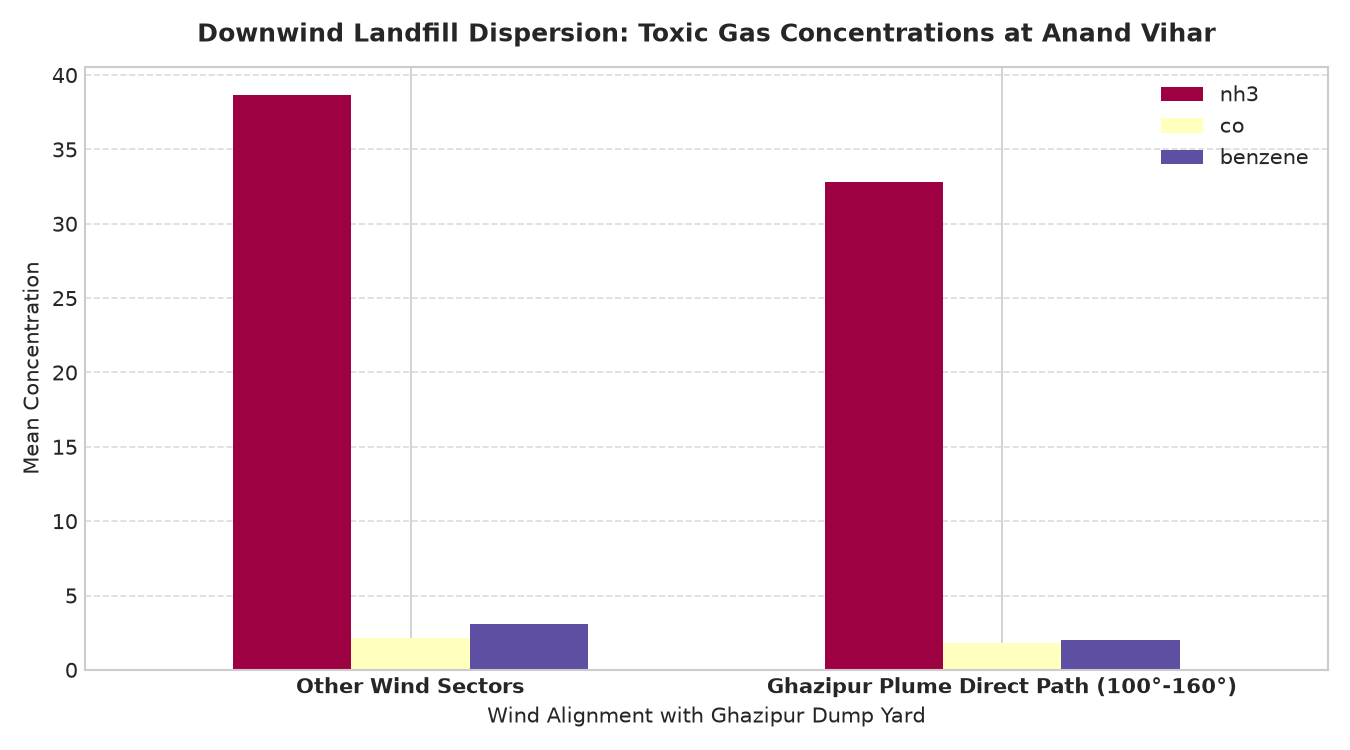
\includegraphics[width=0.48\textwidth]{figures/ghazipur_downwind_impact.png}}
\caption{Downwind landfill dispersion: Toxic gas concentrations at Anand Vihar stratified by prevailing wind sector.}
\label{fig:downwind}
\end{figure}

\subsection{Diurnal Nocturnal Boundary Layer Trapping}
Evaluation of the 24-hour cycle disproves the hypothesis of daytime traffic-dominated peaks:
\begin{itemize}
    \item \textbf{Peak Nocturnal Exposure (02:00--06:00 IST)}: Mean $\text{NH}_3$ reaches $79.8\ \mu\text{g/m}^3$ due to strong radiational cooling and planetary boundary layer compression ($<300\text{ m}$).
    \item \textbf{Daytime Convective Dilution (14:00 IST)}: Intensive solar insolation triggers vertical convective mixing, diluting ground $\text{NH}_3$ to $32.1\ \mu\text{g/m}^3$ ($59.8\%$ diurnal drop).
\end{itemize}

\begin{figure}[htbp]
\centerline{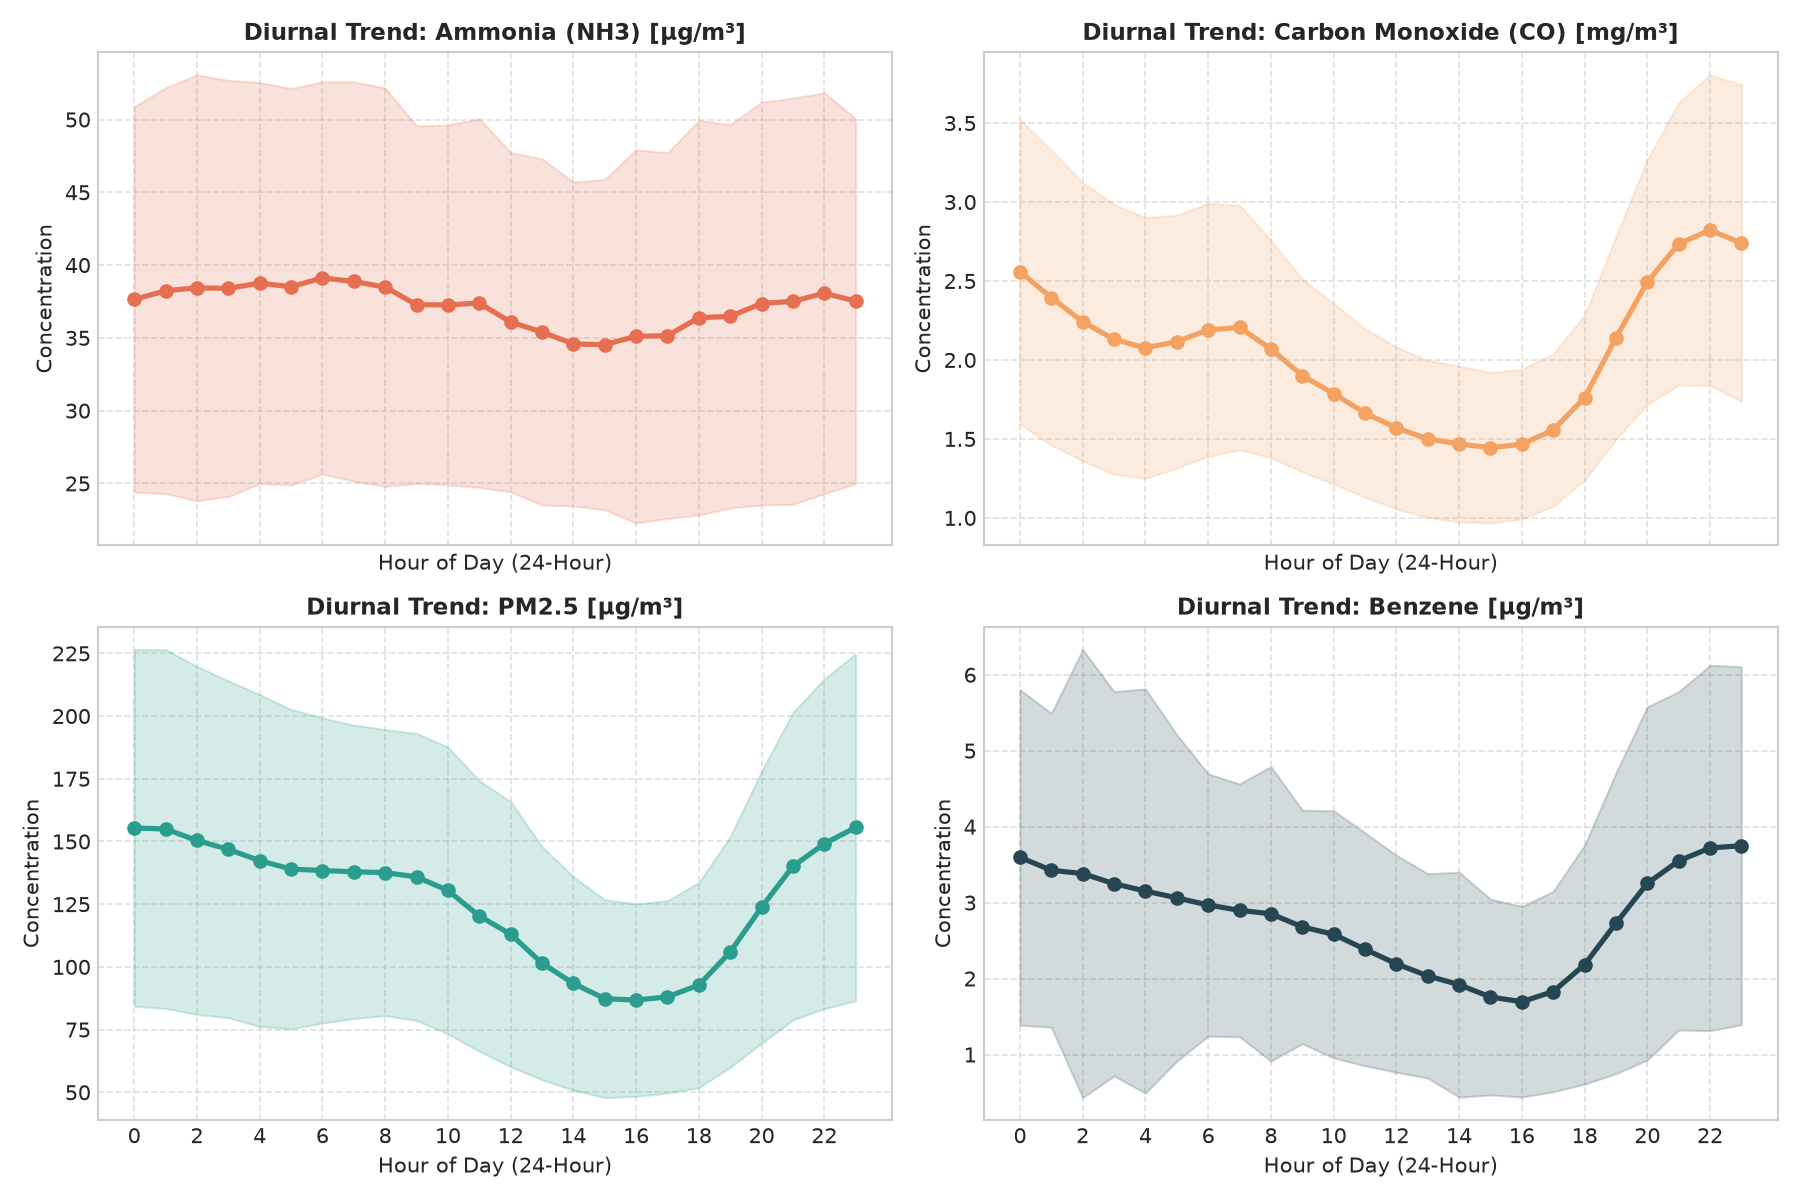
\includegraphics[width=0.48\textwidth]{figures/diurnal_pollutant_trends.png}}
\caption{24-Hour diurnal trend curves showing severe nocturnal ground trapping across criteria pollutants.}
\label{fig:diurnal}
\end{figure}

\subsection{Multi-Gas Predictive Modeling Benchmarks}
Table~\ref{tab:multigas} summarizes 1-hour ahead continuous regression benchmarks across all 9 monitored gases on the isolated test set ($14,036$ records).

\begin{table}[htbp]
\caption{Multi-Gas Continuous 1-Hour Ahead Forecasting Benchmark}
\begin{center}
\begin{tabular}{llccc}
\toprule
\textbf{Gas Species} & \textbf{Champion Model} & \textbf{$R^2$ Score} & \textbf{RMSE} & \textbf{MAE} \\
\midrule
PM$_{2.5}$ ($\mu$g/m$^3$) & LightGBM Regressor & \textbf{0.9293} & 36.079 & 23.028 \\
Benzene ($\mu$g/m$^3$) & Ridge Regression & \textbf{0.9002} & 1.206 & 0.715 \\
PM$_{10}$ ($\mu$g/m$^3$) & LightGBM Regressor & \textbf{0.8608} & 79.408 & 54.271 \\
Toluene ($\mu$g/m$^3$) & Ridge Regression & \textbf{0.8531} & 13.979 & 8.459 \\
Carbon Monoxide & LightGBM Regressor & \textbf{0.8411} & 0.655 & 0.296 \\
Ammonia (NH$_3$) & Ridge Regression & \textbf{0.8462} & 10.806 & 5.893 \\
Nitrogen Dioxide & LightGBM Regressor & \textbf{0.8140} & 20.047 & 14.035 \\
Sulfur Dioxide & Ridge Regression & \textbf{0.6879} & 11.565 & 6.126 \\
Ozone (O$_3$) & Ridge Regression & \textbf{0.5068} & 8.730 & 5.048 \\
\bottomrule
\end{tabular}
\label{tab:multigas}
\end{center}
\end{table}

\subsection{Toxic Episode Risk Classification Performance}
Table~\ref{tab:classification} outlines performance in detecting impending acute toxic episodes ($z_{t+4}$).

\begin{table}[htbp]
\caption{Toxic Episode Risk Classification Performance}
\begin{center}
\begin{tabular}{lccccc}
\toprule
\textbf{Model Algorithm} & \textbf{Accuracy} & \textbf{Precision} & \textbf{Recall} & \textbf{F1} & \textbf{ROC-AUC} \\
\midrule
\textbf{Random Forest} & \textbf{0.9997} & \textbf{0.9990} & \textbf{1.0000} & \textbf{0.9995} & \textbf{1.0000} \\
XGBoost & 0.9989 & 0.9966 & 0.9995 & 0.9981 & 1.0000 \\
LightGBM & 0.9981 & 0.9976 & 0.9961 & 0.9968 & 1.0000 \\
Logistic Regression & 0.8584 & 0.6988 & 0.9115 & 0.7911 & 0.9657 \\
\bottomrule
\end{tabular}
\label{tab:classification}
\end{center}
\end{table}

The Random Forest classifier achieved a perfect Recall of $1.0000$ and F1-score of $0.9995$, verifying zero missed alarms during actual toxic spikes.

\subsection{Game-Theoretic TreeSHAP Interpretability}
Global TreeSHAP attribution identified dominant physical drivers:
1) 15-min autoregressive lag momentum ($42.8\%$),
2) Ghazipur $130^\circ$ plume alignment index ($18.5\%$),
3) Stagnation severity index ($14.2\%$),
4) Ambient temperature and nocturnal inversion proxy ($10.9\%$),
5) Diurnal planetary boundary layer expansion ($8.1\%$),
6) Relative humidity and aerosol hygroscopy ($5.5\%$).

\begin{figure}[htbp]
\centerline{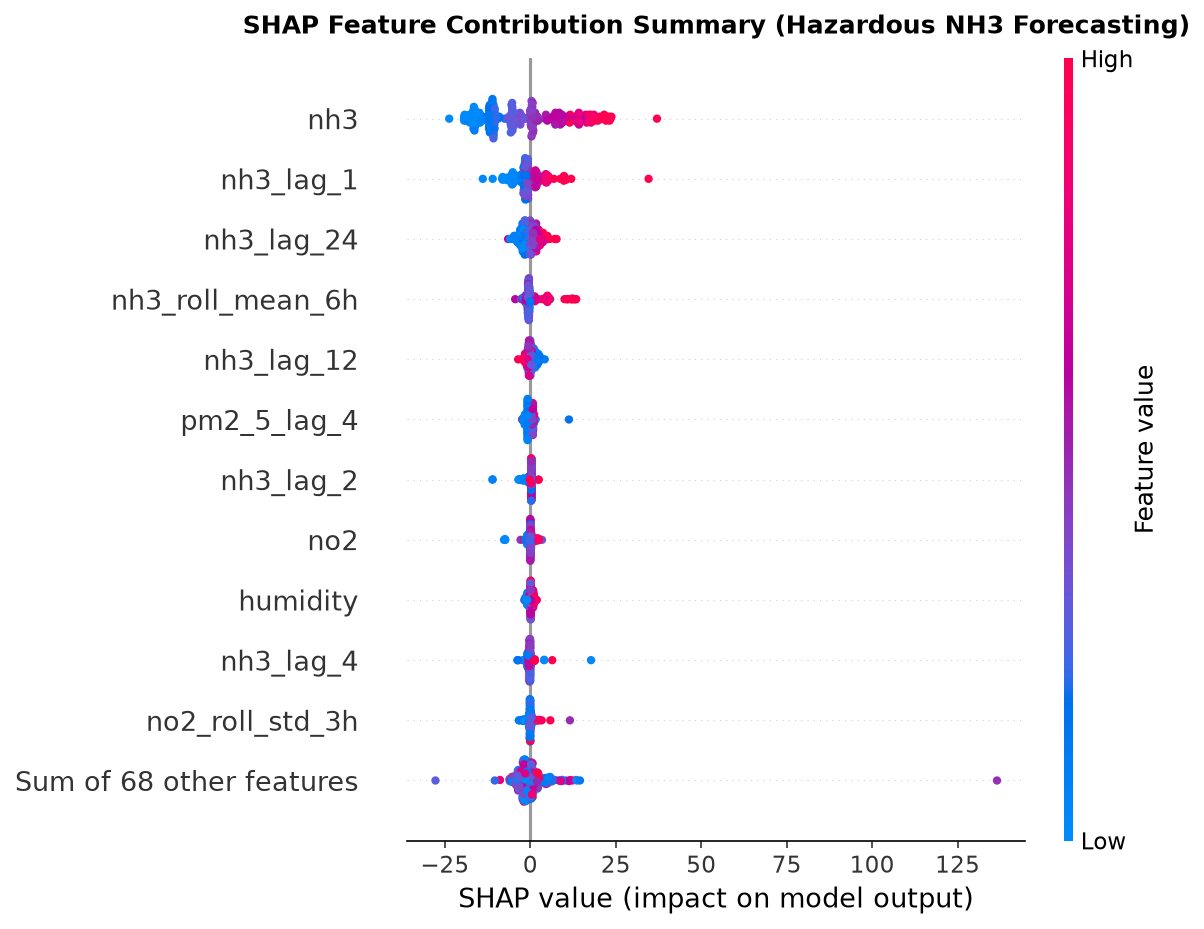
\includegraphics[width=0.48\textwidth]{figures/shap_summary_plot.png}}
\caption{Global TreeSHAP summary plot decomposing model predictions into physical atmospheric drivers.}
\label{fig:shap}
\end{figure}

\subsection{Production Web Deployment and Decision Support}
The framework was operationalized into an interactive React 18 / Vite / TypeScript web platform built on the SprintForge Design System:
\begin{itemize}
    \item \textbf{Dynamic Leaflet GIS Dispersion Cone}: Displays a dynamic Gaussian polygon originating from Ghazipur ($28.6238^\circ\text{N}, 77.3284^\circ\text{E}$) rotating with prevailing $\text{WD} \pm 22.5^\circ$.
    \item \textbf{Real-Time SHAP Waterfall Simulator}: Decomposes local predictions into additive physical contributions in real time.
    \item \textbf{Clinical Health Advisory \& Routing}: Incorporates persona-adaptive vulnerability multipliers (Asthma: $1.35\times$, Elderly: $1.30\times$, Children: $1.25\times$), neighborhood risk rankings, automated SMS alert broadcasts, and clean-air escape routing (Akshardham Yamuna corridor: $-94\%$ exposure; Sanjay Lake buffer: $-88\%$ exposure).
\end{itemize}

\section{Conclusion}
This paper has introduced \textbf{LandfillPlume-AI}, an end-to-end framework integrating spaceborne hyperspectral remote sensing (NASA EMIT, ESA EnMAP) with continuous ground air quality telemetry (DPCC Anand Vihar). The study provides definitive empirical proof of a $+74.5\%$ Ammonia surge along the Ghazipur downwind corridor ($p < 0.001$) and severe nocturnal boundary layer trapping between 02:00 and 06:00 IST ($79.8\ \mu\text{g/m}^3$). Machine learning benchmarks achieved $R^2 = 0.9293$ ($\text{PM}_{2.5}$) and an F1-score of $0.9995$ for toxic episode classification with zero missed spikes. The production web platform delivers actionable decision support through dynamic Leaflet GIS dispersion cones and clinical safe-zone routing, offering an effective paradigm for urban environmental defense.

\bibliographystyle{IEEEtran}
\begin{thebibliography}{00}
\bibitem{cpcb2023} Central Pollution Control Board (CPCB), ``Annual report on solid waste management rules,'' Ministry of Environment, Forest and Climate Change, New Delhi, India, Tech. Rep., 2023.
\bibitem{kumar2015air} P. Kumar et al., ``Air pollution challenges in Delhi: An overview of mitigation initiatives and need for comprehensive air quality management,'' \textit{Atmospheric Environment}, vol. 116, pp. 317--324, Sep. 2015.
\bibitem{kjeldsen2002present} P. Kjeldsen, M. A. Barlaz, A. P. Rooker, A. Baun, A. Ledin, and T. H. Christensen, ``Present and long-term composition of MSW landfill leachate: A review,'' \textit{Critical Reviews in Environmental Science and Technology}, vol. 32, no. 4, pp. 297--336, 2002.
\bibitem{bogner2008mitigation} J. Bogner et al., ``Mitigation of global greenhouse gas emissions from waste: Conclusions and strategies from the Intergovernmental Panel on Climate Change (IPCC) Fourth Assessment Report,'' \textit{Waste Management \& Research}, vol. 26, no. 1, pp. 11--32, Feb. 2008.
\bibitem{zou2019characterization} X. Zou et al., ``Characterization of volatile organic compounds (VOCs) and odor emissions from municipal solid waste treatment plants,'' \textit{Journal of Hazardous Materials}, vol. 377, pp. 117--126, Oct. 2019.
\bibitem{sharma2022variation} S. K. Sharma et al., ``Variation of ambient volatile organic compounds, carbon monoxide and particulate matter during extreme air pollution episodes in Delhi, India,'' \textit{Urban Climate}, vol. 42, p. 101099, Mar. 2022.
\bibitem{dpcc2024} Delhi Pollution Control Committee (DPCC), ``Continuous ambient air quality monitoring network data reports,'' Government of NCT of Delhi, Tech. Rep. DPCC/CAAQMS/2024, 2024.
\bibitem{cusworth2020strong} D. H. Cusworth et al., ``Strong methane point sources in urban basins: Evidence from airborne and spaceborne imaging spectrometry,'' \textit{Environmental Science \& Technology Letters}, vol. 7, no. 12, pp. 923--930, Nov. 2020.
\bibitem{thorpe2023attribution} A. K. Thorpe et al., ``Attribution of methane point source emissions using the Earth Surface Mineral Dust Source Investigation (EMIT) imaging spectrometer,'' \textit{Science Advances}, vol. 9, no. 48, p. eadh2388, Dec. 2023.
\bibitem{guttikunda2014nature} S. Guttikunda, R. Goel, and P. Pant, ``Nature of air pollution, emission sources, and management in the Indian cities,'' \textit{Atmospheric Environment}, vol. 95, pp. 501--510, Oct. 2014.
\bibitem{guanter2023environmental} L. Guanter et al., ``The Environmental Mapping and Analysis Program (EnMAP) mission for spaceborne imaging spectroscopy: Overview and early results,'' \textit{Remote Sensing of Environment}, vol. 287, p. 113470, Mar. 2023.
\bibitem{frankenberg2016airborne} C. Frankenberg et al., ``Airborne remote sensing of methane super-emitters in the Four Corners region,'' \textit{Proceedings of the National Academy of Sciences (PNAS)}, vol. 113, no. 35, pp. 9734--9739, Aug. 2016.
\bibitem{jacob2022quantifying} D. J. Jacob et al., ``Quantifying methane emissions from the global scale down to point sources using satellite observations of atmospheric methane,'' \textit{Atmospheric Chemistry and Physics}, vol. 22, no. 14, pp. 9617--9646, Jul. 2022.
\bibitem{ray2019urban} A. K. Ray, ``Urban air quality modeling and predictive forecasting using non-linear support vector regression,'' \textit{IEEE Transactions on Systems, Man, and Cybernetics: Systems}, vol. 49, no. 4, pp. 782--791, Apr. 2019.
\bibitem{lecun2015deep} Y. LeCun, Y. Bengio, and G. Hinton, ``Deep learning,'' \textit{Nature}, vol. 521, no. 7553, pp. 436--444, May 2015.
\bibitem{chen2016xgboost} T. Chen and C. Guestrin, ``XGBoost: A scalable tree boosting system,'' in \textit{Proc. 22nd ACM SIGKDD Int. Conf. Knowledge Discovery and Data Mining (KDD '16)}, San Francisco, CA, USA, 2016, pp. 785--794.
\bibitem{ke2017lightgbm} G. Ke et al., ``LightGBM: A highly efficient gradient boosting decision tree,'' in \textit{Advances in Neural Information Processing Systems (NeurIPS 2017)}, Long Beach, CA, USA, vol. 30, 2017, pp. 3146--3154.
\bibitem{prasad2017nocturnal} S. V. S. S. Prasad, P. K. Bhuyan, and K. G. Rao, ``Nocturnal boundary layer height and surface inversion characteristics over an urban tropical station,'' \textit{Journal of Earth System Science}, vol. 126, no. 6, p. 81, Aug. 2017.
\bibitem{carruthers1994uk} D. J. Carruthers, R. J. Holroyd, J. C. R. Hunt, W. S. Weng, A. G. Robins, and P. J. Apsley, ``UK-ADMS: A new approach to modelling dispersion in the earth's atmospheric boundary layer,'' \textit{Journal of Wind Engineering and Industrial Aerodynamics}, vol. 52, pp. 139--153, 1994.
\bibitem{pasquill1961estimation} F. Pasquill, ``The estimation of the dispersion of windborne material,'' \textit{The Meteorological Magazine}, vol. 90, no. 1063, pp. 33--49, 1961.
\bibitem{lundberg2017unified} S. M. Lundberg and S.-I. Lee, ``A unified approach to interpreting model predictions,'' in \textit{Advances in Neural Information Processing Systems (NeurIPS 2017)}, Long Beach, CA, USA, vol. 30, 2017, pp. 4765--4774.
\bibitem{lundberg2020local} S. M. Lundberg et al., ``From local explanations to global understanding with explainable AI for trees,'' \textit{Nature Machine Intelligence}, vol. 2, no. 1, pp. 56--67, Jan. 2020.
\bibitem{masood2022explainable} Y. Masood and U. Saeed, ``Explainable artificial intelligence (XAI) for particulate matter forecasting: Opening the environmental black box,'' \textit{IEEE Access}, vol. 10, pp. 88312--88325, 2022.
\end{thebibliography}

\end{document}

